\documentclass[11pt, british]{beamer}

\usetheme{metropolis}
\usepackage{appendixnumberbeamer}

\usepackage{default}
\usepackage{booktabs}
\usepackage{graphicx}
\usepackage{svg}
\usepackage[scale=2]{ccicons}
\usepackage[utf8]{inputenc}

\usepackage{pgfplots}

%\usepgfplotslibrary{dateplot}
\usepackage{csquotes}
\usepackage[backend=bibtex8, style=authoryear]{biblatex}
\bibliography{biblio}

\usepackage{verbatim}
\usepackage{xspace}

\newrobustcmd*{\parentexttrack}[1]{%
	\begingroup
	\blx@blxinit
	\blx@setsfcodes
	\blx@bibopenparen#1\blx@bibcloseparen
	\endgroup}

\AtEveryCite{%
	\let\parentext=\parentexttrack%
	\let\bibopenparen=\bibopenbracket%
	\let\bibcloseparen=\bibclosebracket}

\title{Big Data and Big Privacy}
\subtitle{Finding an equilibrium}
\date{28th November 2017}
\author{Francesco Picciotti}
\institute{Computer Ethics (2017-18), Politecnico di Milano}

\begin{document}
	
	\maketitle

	\begin{frame}{Central idea}
		The aim of the presentation is to show that:
		\begin{itemize}
			\item Privacy cannot be \textbf{downplayed} or traded for having 
			\textbf{better services}
			\item Existing solutions are \textbf{not enough}
			\item Propose \textbf{a new perspective} for finding new solutions, 
			as a \alert{constructive tradeoff} in which both sides 
			\textbf{collaborates} to achieve \textbf{convenient results} for 
			both    
		\end{itemize}
	\end{frame}
	
	\begin{frame}{Outline}
		\setbeamertemplate{section in toc}[sections numbered]
		\tableofcontents[hideallsubsections]
	\end{frame}
	
	\section{Introduction to Big Data}
	\begin{comment}
	\begin{frame}{What is Big Data?}
		\begin{displayquote}
		"Big data is high volume, high velocity, and/or high variety 
		information assets that require new forms of processing to enable 
		enhanced decision making, insight discovery and process optimization"
		\end{displayquote}
	\end{frame}
	
	\begin{frame}{In a nutshell}
		\begin{figure}
		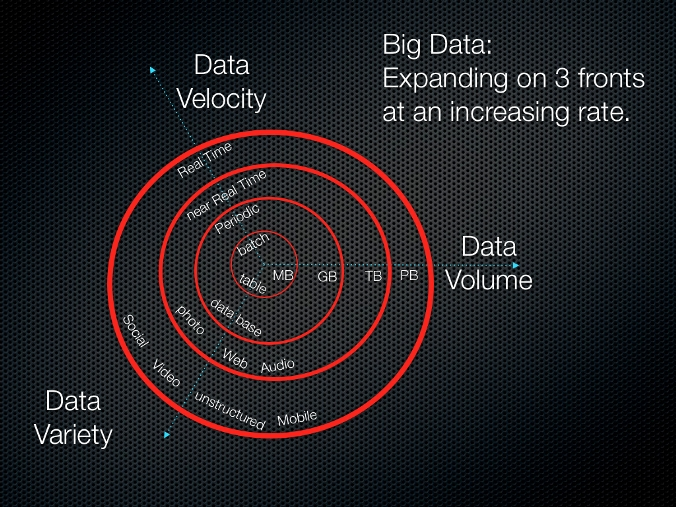
\includegraphics[width=0.9\textwidth]{./Imgs/BigData001.jpg}
		\caption{\cite{1}}
		\end{figure}
	\end{frame}
	\end{comment}
	
	\begin{frame}{The reason of the rise}
			The Big Data happening is a \textbf{combination} of two 
			technologies growth during the last 30 years:
		\begin{itemize}
			\item A significant \alert{paradigm-shift} of AI
			\item Development of a big and unified \alert{data infrastructure}
		\end{itemize}
		As a matter of fact, the \alert{huge amount of data} daily produced by 
		us is now easily \textbf{stored} and \textbf{available for other 
		purposes}.
	\end{frame}
	
	\begin{frame}{The Devil's in the... numbers}
		\begin{itemize}
			\item \alert{Amazon.com} handles millions of back-end operations 
			every day, 
			as well as queries from \textbf{more than half a million 
				third-party 
				sellers}. \parencite{1}
			\item \alert{Facebook} handles \textbf{50 billion photos} from its 
			user 
			base. \parencite{2} 
			\item \alert{Google} was handling roughly \textbf{100 billion 
				searches per month} as of August 2012. \parencite{3} 	
		\end{itemize}
	\end{frame}
	
	\section{Case study: The Big G services}
	
	\begin{frame}{What is happening?}
		\begin{figure}
			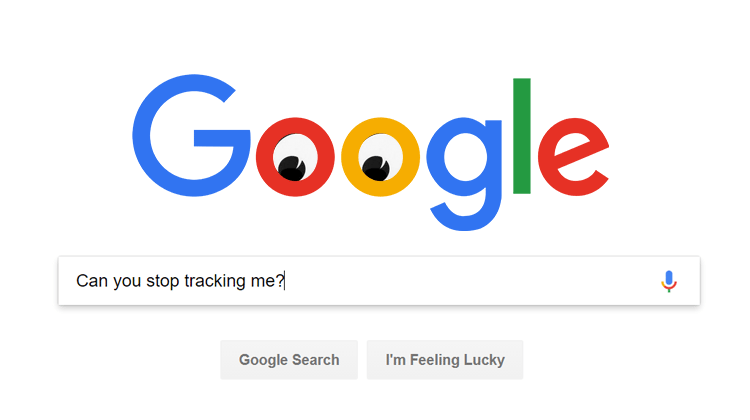
\includegraphics[width=1\textwidth]{./Imgs/Prevent-Google-Tracking.png}
			\caption{From \parencite{4}}
		\end{figure}
	\end{frame}
	
	\begin{frame}{Behind the daily interaction with Google}
		Without any doubt \alert{Google} is the most pervasive company, just 
		think about of the \textbf{daily usage of services} in our 
		\textbf{smartphones}.
		
		\begin{alertblock}{Search Engine}
			The most known SEO stores permanently our \textbf{web searches}, 
			monitoring 
			our \textbf{interests} and \textbf{behaviors}. 
		\end{alertblock}

		\begin{alertblock}{Gmail}
			When we use the company's email services, Google \textbf{scans our 
			emails}, 
			as well as the \textbf{recipients}. 
		\end{alertblock}		
	\end{frame}
	
	\begin{frame}{Behind the daily interaction with Google (cont'd)}
		\begin{alertblock}{Google Maps}
			 If you have location history enabled then Google knows the 
			 \textbf{places 
			 that you hang out} or where you \textbf{travel to}.   
		\end{alertblock}
		
		\begin{alertblock}{Google Photos}
			When you upload your photos, you are giving the tech giant license 
			to \emph{"host, store, reproduce, modify, create derivative works, 
			communicate, publish, publicly perform, publicly display and 
			distribute"} [Google’s Terms of Service] those photos   
		\end{alertblock}
	...and there are \textbf{plenty other services} and they are all \alert{for 
	free}.		
	\end{frame}
	
	\section{The Big Issue}
	
		\begin{frame}{What is the problem?}
			It looks like we have to allow the \textbf{collection of our 
			personal informations}.
			\\ 
			One may say:
			\begin{itemize}
				\item The Google's data gathering implies a 
				\textbf{significant improvement} 
				of service
				\item The disclosure of personal 
				information is \textbf{restricted}
				\item \textbf{Overconcern} about \alert{privacy}
			\end{itemize}
		\end{frame}
		
		\begin{frame}{The problem is the Price}
			\begin{figure}
				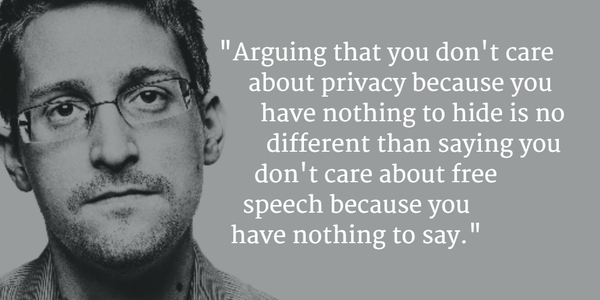
\includegraphics[width=\linewidth]{Imgs/snowden.png}
				\caption{Edward Snowden's quote}
			\end{figure}
		\end{frame}
		
		\begin{frame}{The Price}
			The main reasons about the \textbf{preciousness} of our personal 
			informations are 
			conveyed by \parencite{5} :
			\begin{itemize}
				\item Protect \alert{people's interest}
				\item \alert{Hide aspect of life} or behavior that would be 
				\textbf{embarrassing} to disclose
				\item \alert{Confidentiality}
				\item \alert{Avoid to be judged} with \textbf{unrelated} facts
				\item \alert{Control} of the access to \textbf{personal 
				information}
			\end{itemize}
		\end{frame}
		
		\begin{frame}{The social valence}
			The relevance as \textbf{social good} depicted by the several 
			aspects \parencite{6} :
			\begin{itemize}
				\item \alert{Common value}, reframing privacy towards an
				\textbf{utilitarian view} (i.e. Privacy vs Security)
				\item \alert{Public value}, necessary to \textbf{support 
				democratic 
				processes} and to the \textbf{forming of a body politic} or 
				public (i.e. Ads targeting during Trump presidential campaign)
				\item \alert{Collective value}, privacy \textbf{protecting the 
				common pool} of personal informations (i.e. Data Breach)  
			\end{itemize}
		\end{frame}
		
		\begin{frame}{The Contextual integrity valence}
			It is even clearer once considered as \alert{Contextual Integrity} 
			\parencite{7}, information flows according to:  
			\begin{itemize}
				\item \textbf{Key actors}
				\item \textbf{Types of information}
				\item Constraints under which flow occurs 
				(\textbf{Transmission}) 
			\end{itemize}
		\end{frame}

\begin{comment}	
		\begin{frame}{}
			The privacy issue has a great importance because:
			depicted	
			\begin{itemize}
				\item Differente valenza della privacy
				\item Data leak and hacking
				\item Uso non trasparente dei dati perchè viene utilizzata 
				anche per scopi commerciali e di sorveglianza 
				\item Non possiamo sacrificarla per buoni servizi 
			\end{itemize}
		\end{frame}
\end{comment}		
	
		\begin{frame}{The miracle cure?}
			%Informed consent, anonimization,
			The existing ways to shield the privacy of users, according to 
			\parencite{8}, are:
			\begin{itemize}
				\item \alert{Anonymity}: \textbf{Hide identities} 
				(\textbf{PII}, 
				thus  Personally Identifiable Informations) from the records 
				using a \textbf{unique persistent identifier} (i.e. Google's 
				anonymous identifier is AdID)
				\item \alert{Informed Consent}: Make users informed \textbf{who 
				is collecting data}, if the \textbf{data collection is 
				compulsory}, how \textbf{information} is \textbf{used} and 
				\textbf{shared}
			\end{itemize} 
		\end{frame}
		
		\begin{frame}{Limits}
			\begin{alertblock}{Anonymity}
				\begin{itemize}
					\item \alert{Linkage Attack}: An attacker can retrieve the 
					identifying information \textbf{joining} the anonymized 
					dataset with another one with identities
					\item \alert{Differencing Attack}: Performing a sequence of 
					queries on anonymized dataset, the attacker \textbf{can 
					deduce} a certain person \textbf{is} in the dataset
					\item \alert{Pseudonymity}: Even without knowing the 
					\textbf{person's name}, company knows the user's behavior 
					and tastes  
				\end{itemize}
			\end{alertblock}
		\end{frame}
		
		\begin{frame}{Limits cont'd}
			\begin{alertblock}{Informed Consent}
				\begin{itemize}
					\item \alert{Transparency Paradox}: Simplicity and clarity 
					results in \textbf{losses of fidelity}, therefore they have 
					some degree of \textbf{obscurity} to hide violations
					\item \alert{Unpredictable}: There are no 
					\textbf{guarantees} on how much \textbf{time} the 
					information will flow, who will \textbf{use} and work 
					on these data
					\item \alert{Opt-out} conditions, in order to use the 
					service the user must \textbf{accept} the terms
				\end{itemize}
			\end{alertblock}
		\end{frame}
		
	\section{The Big Challenge}
	
		\begin{frame}{The situation}
			\begin{figure}
				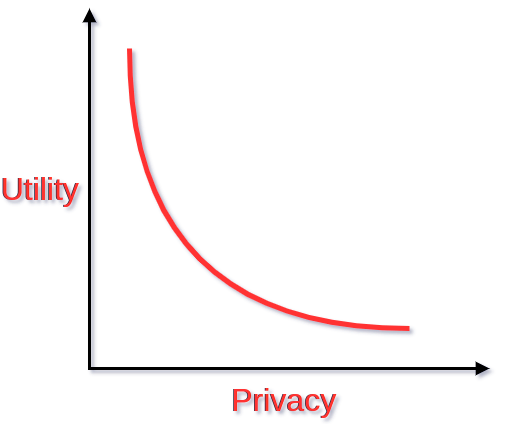
\includegraphics[width= 0.8\linewidth]{Imgs/Tradeoff.png}
				\caption{Inspired from \parencite{9}}
			\end{figure}
		\end{frame}
	
		\begin{frame}{Pushing the boundary up}
			\begin{figure}
				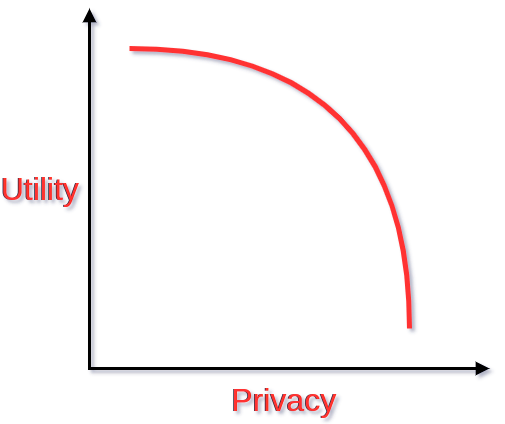
\includegraphics[width= 0.8\linewidth]{Imgs/SwapTradeoff.png}
				\caption{Inspired from \parencite{9}}
			\end{figure}
		\end{frame}
	
		\begin{frame}{Est modus in rebus: From the company's perspective}
				\begin{itemize}
					\item Anonymity implementations has to be \textbf{improved} 
					and also 
					apply \textbf{data perturbation}
					\item The Informed Consent has to be at least clearer, but 
					generally it is \textbf{inadequate}
					\item Reduce the damages of data breaches and leaks 
					avoiding a \textbf{single point of failure}, using:
					\begin{itemize}
						\item \textbf{Segmentation}, switching from big data to 
						\textbf{small local data} 
						\item \textbf{Encryption} of data
					\end{itemize}
					\item The willingness to give \textbf{some profit} up and 
					put more effort on finding \textbf{concrete} and 
					\textbf{adequate} solution
				\end{itemize}
		\end{frame}
			
		\begin{frame}{Est modus in rebus: From the user's perspective}
				\begin{itemize}
					\item Basic notions of privacy and \textbf{how to protect 
					it} (i.e. How to prevent Google tracking on any browser 
					\parencite{4})
					\item Increased \textbf{responsibility} about the usage of 
					some tools or services
					\item More \textbf{awareness} on the existence of other 
					\textbf{alternatives}
					\item \textbf{Consciousness} of the informed consent in 
					which we “agree” on
					\item \textbf{Limiting the usage} of some technologies 
					depending on the purpose (i.e. GPS tracking activities)
				\end{itemize}
		\end{frame}
		
		\begin{frame}{The Devil's in the... details}
			\begin{figure}
				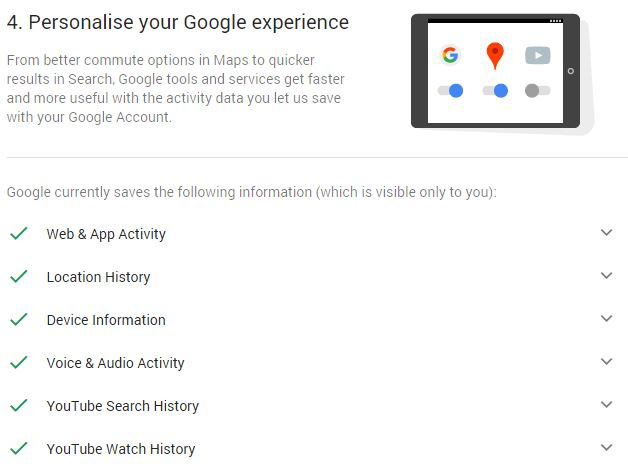
\includegraphics[width=\linewidth]{Imgs/google-privacy-checkup.jpg}
			\end{figure}
		\end{frame}
		
		\begin{frame}{The need for an alternative}
			\begin{figure}
				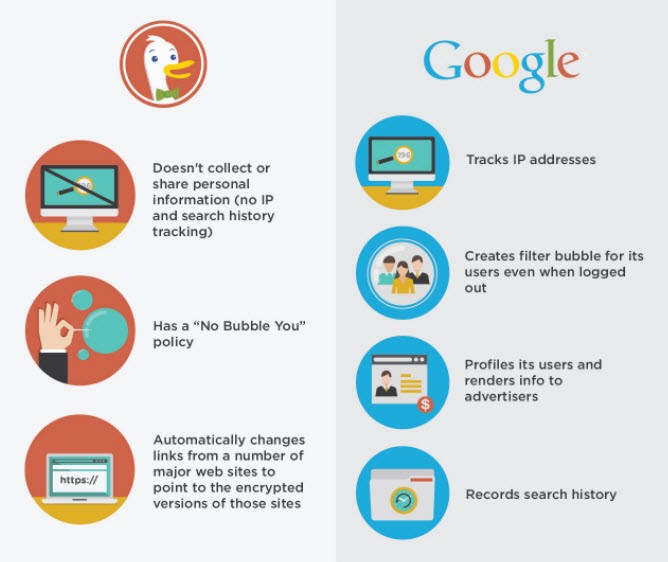
\includegraphics[width=0.9\linewidth]{Imgs/hackernoon.jpeg}
			\end{figure}
		\end{frame}
		
		\begin{frame}[standout]
			\begin{displayquote}
				"Be the change that you wish to see in the world." 
				\flushright{Mahatma Gandhi}
			\end{displayquote}
			Thanks for your attention
			\\
			Questions?
		\end{frame}
	
		\begin{frame}[allowframebreaks]
			\printbibliography
		\end{frame}
	
\end{document}
